\documentclass[letterpaper]{article}
\usepackage{amsmath}
\usepackage{amsfonts} % for \mathbb{R}
\usepackage{amssymb} % for \triangleq
\usepackage{alg}
\usepackage{booktabs} % for table setting
\usepackage[pdftex]{graphicx}
\usepackage[margin=1.2in]{geometry}


\begin{document}
\thispagestyle{empty}
\pagestyle{empty} % no page numbers

\author{Dylan Hutchison}
\title{A Comparison between Dempster-Shafer and Bayesian Approaches to Soft Evidence}
\date{last updated \today}
%\institute{Stevens Institute of Technology\\
%Hoboken, NJ 07030
%\email{dhutchis@stevens.edu}}
\maketitle

%\noindent Dylan Hutchison\\
%CS 810B Causal Inference\\
%Project Proposal due 29 October 2012
%\begin{center}
%A Comparison between Dempster-Shafer and Bayesian Approaches to Soft Evidence
%\end{center}

\section{Probability and Dempster-Shafer}
Let $X$ be a random variable and $D_X$ be the domain of X (the possible states X can assume).  Traditional probability theory assigns a weight to each state $x \in D_X$, denoted as $P(X=x)$ (or just $P(x)$ when $X$ is understood as the random variable) such that $\sum_{x \in D_X}x = 1$. Ideally, $P(X=x)$ will equal the long run proportion 
\[P(X=x) = \dfrac{\text{the true \# of possible worlds where } X=x}{\text{total \# of possible worlds}}\]
In the non-ideal case, $P(x)$ is our best guess of the above true long run proportion.

Dempster-Shafer theory\footnote{see \cite{Shafer1976} for the comprehensive presentation of Dempster-Shafer theory with proofs} assigns probability \textit{masses} to each subset $A \in 2^X$, where $2^X$ is the power set of $D_X$ and $m(A)$ is the mass assignment, with the similar requirement that $\sum_{A \in 2^{X}}m(A) = 1$.  One can think of the probability mass as an assignment of probability to a set of possible worlds.  
From the probability mass we derive the useful \textit{belief} $Bel$ and \textit{plausibility} $Pl$ functions, defined as:
\[
\begin{array}{rl}
Bel(A) & \triangleq \text{sum of masses of subsets of A}\\
	& = \sum_{B \subseteq A} m(B) \\
	& = \dfrac{\text{\# of worlds where A \textbf{provably} contains the truth}}{\text{total \# of worlds}}\\
	& = \text{a very conservative lower bound on } P(A)\\
Pl(A) & \triangleq 1-Bel(\bar{A})\\
	& = 1-\dfrac{\text{\# of worlds where A \textbf{provably never} contains the truth}}{\text{total \# of worlds}}\\
	& = \text{a very conservative upper bound on } P(A)\\
Pl(A)-Bel(A) & = \dfrac{\text{\# of worlds where A \textbf{possibly} contains the truth}}{\text{total \# of worlds}}\\
	& = \text{our range of uncertainty that the truth lies in } A
\end{array}
\]
As an axiom, $m(\emptyset)=Bel(\emptyset)=0$, and we can derive that $Bel(D_X)=1$.  Perhaps the best way to describe these functions and their properties is by example, so let's move on to a simple example.
%and so the reader may want to skip to the next section to gain familiarity with manipulating masses.

\section{D.S. by Example: 2-State Single Variable}
\subsection{No evidence}
Suppose someone gives hands you a coin, but tells you nothing about the nature of the coin.  It could be oddly weighted, favoring heads more than tails or vice versa, or it could be fair.  Under Dempster-Shafer tenets, we would assign the \textit{vacuous} belief function (vacuous because it represents no information)
\[ m(\{Heads\}) = 0, m(\{Tails\}) = 0, m(\{Heads,Tails\})=1 \]
and impart the following beliefs and plausibilities found in Table~\ref{tab:CoinFlipNoInfo}.

\begin{table}[htbp]
\centering
\caption{Coin flip with no information}
\begin{tabular}{rcccc}
\toprule
                subset&mass &bel  &Prob &plaus\\
\midrule
                    {[]}&0    &0    &     &0    \\
               {[Heads]}&0    &0    &0.5  &1    \\
               {[Tails]}&0    &0    &0.5  &1    \\
        {[Heads, Tails]}&1    &1    &     &1    \\
\bottomrule
\end{tabular}
\label{tab:CoinFlipNoInfo}
\end{table}

As expected, the belief (lower bound on the probability) of each single event is 0 and the plausibility (upper bound on probability) of each single event is 1.  We have no information at all on the true probability of the event, as we see from the uncertainty $Pl(a)-Bel(a)=1$ for $a=\{Heads\},\{Tails\}$.  However, we have total certainty that the probability for $A=\{Heads,Tails\}$, i.e., we know that $P(A)=1$ with uncertainty $1-1=0$ because there are no other values the coin state could take on (no sideways landings, etc.). All worlds must have a state for the coin flip in the subset $\{Heads,Tails\}$.

\subsection{Deriving probability from the masses}
But how might we obtain the probability of an event, such as $P(Heads)$?  We know that $0 \leq P(Heads) \leq 1$, but that's not very useful information. We need to make an assumption essential to Bayesian reasoning: \emph{assume equal probability in the absence of additional information}.  We can do that by breaking up the mass assigned to subsets of more than one element among its constituent elements.  Here, we can divide m(\{Heads,Tails\}) among its 2 components and assign $P(Heads)=0.5$ and $P(Tails)=0.5$.  Here is the general case $\forall a \in D_X$:
\[ P(a) = \sum_{B:\; a \in B \subseteq 2^X}\frac{m(B)}{|B|} \]
In future tables, I will include probability estimates derived by this rule under the heading \textsc{prob}.

\subsection{Certain evidence}
After examining the coin given to us, we discover that it has heads on both sides!  We can account for this new information by creating a new mass distribution shown in Table~\ref{tab:CoinFlipAllHeads}.\footnote{Technically we need to combine the mass function representing the new evidence with the mass function representing our previous state of belief using Dempster's Rule of Combination to arrive at a new, updated state of belief, but I will omit the combination for now because combining evidence with the vacuous belief state trivially replaces the vacuous mass with the evidence mass.}
Notice that the level of uncertainty in the events $a \in D_X$ is $Pl(\{a\})-Bel(\{a\})=0$.  We say we have a \textit{complete} probability specification for the variable whenever this is the case.  

\begin{table}[htbp]
\centering
\caption{Always-heads coin flip}
\begin{tabular}{rcccc}
\toprule
                subset&mass &bel  &Prob &plaus\\
\midrule
                    {[]}&0    &0    &     &0    \\
               {[Heads]}&1    &1    &1    &1    \\
               {[Tails]}&0    &0    &0    &0    \\
        {[Heads, Tails]}&0    &1    &     &1    \\
\bottomrule
\end{tabular}
\label{tab:CoinFlipAllHeads}
\end{table}

\subsection{Weakening evidence}
Now let's look at another coin with a heads side and tails side, but still no knowledge of any weighting it may have.  Suppose we weigh the coin on a scale which concludes that uneven weight distributions in the coin give it a 70\% chance of Heads.  However, there is uncertainty in the evidence since the magnetometer may be faulty or there may be other sources of bias in the coin (such as magnetism), allowing us to trust the evidence with only 60\% confidence.  How can we weaken the traditional assignment $\{ m(\{Heads\})=0.7, m(\{Tails\})=0.3 \}$ so that we leave some level of uncertainty in our probabilities?  We need to find some function f with parameter c (our level of confidence) and the following properties:
\begin{itemize}
\item The masses are unaltered (not weakened) when c = 1.
\item The masses become the vacuous function when c = 0, destroying any information the evidence originally bore.
\item The strength of the evidence varies linearly\footnote{Why linear? Because we have no reason not to use a linear relationship and, as a guideline, simpler models are better than complex ones.} with c. % Cite someone who said this?
\end{itemize}
I propose the following \textit{weakening function} to meet these requirements:
\[ f(m(A),c) = \begin{cases}
	m(A)*c &\mbox{if } A \neq D_X\\
	m(A)+(1-c) &\mbox{if } A = D_X \end{cases}
\]
It reads, ``Take away from each informative subset a factor of confidence c and add the total taken away to the uninformative all-event-set." The following figures demonstrate the effects of the weakening function on a random variable of domain size 3 (not related to the coin flipping example!) and probabilities 0.05, 0.80 and 0.15.
% Todo: add legend matching color to probability (or prob. ratio for 2nd figure)

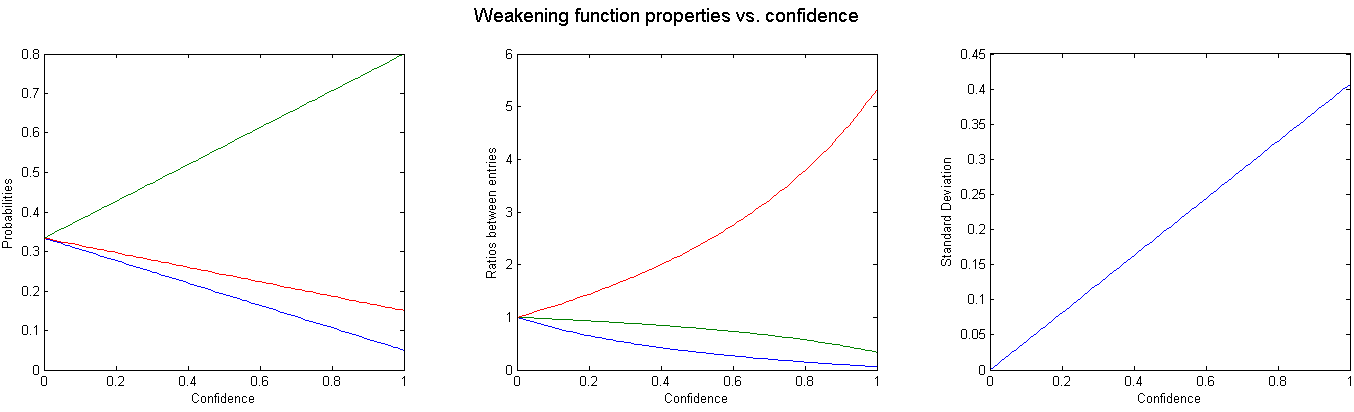
\includegraphics[width=\linewidth]{WeakeningFunctionExamplePlots.png}
% TODO:
\textsc{What should I say about the nonlinear decrease of the ratios of the probabilities nonlinearly approaching unity?}
From the left plot, we see that the weakening function matches all three properties.  It also has the good property of linearly reducing the standard deviation of the probabilities as shown in the right plot.

Let's return to our coin flipping example and apply the weakening function.  We arrive at the mass distribution in Table~\ref{tab:CoinFlipWeakened}.  The results fit exactly what we expect: an uncertainty of $Pl(\{a\})-Bel(\{a\})=0.4$ and a probability shifted from the original value of 0.5 60\% of the way toward the evidential value of 0.7.
\begin{table}[htbp]
\centering
\caption{7:3 evidence in favor of Heads, weakened by 60\% certainty}
\begin{tabular}{rllll}
\toprule
                subset&mass &bel  &Prob &plaus\\
\midrule
                    {[]}&0    &0    &     &0    \\
               {[Heads]}&0.420&0.420&0.620&0.820\\
               {[Tails]}&0.180&0.180&0.380&0.580\\
        {[Heads, Tails]}&0.400&1    &     &1    \\
\bottomrule
\end{tabular}
\label{tab:CoinFlipWeakened}
\end{table}

\subsection{Combining Evidence}
Now that we have examined two types of evidence, the natural next step is to ask how to combine them after observing both.  We can predict the outcome in advance; combining knowledge that the coin will always flip to heads and knowledge with 60\% certainty that Heads will appear 70\% of the time ought to result in knowledge that the coin will always flip to heads.  More generally, we can show that a complete probability model will always remain a complete probability model when combined with any evidence. (Todo CITE this result, or provide it here // and this may not be the right place as it gives the impression that the certain evidence cannot change (only true here because all our mass is on Heads))

Let $m_1$ and $m_2$ be the first and second piece of evidence forming the resultant probability mass $m_{1 \oplus 2}$.  We must consider every pairing of masses for each subset $\in 2^X$.  There are three cases of evidence combination:
\begin{itemize}
\item Evidence in total agreement. Apply the combination of $m_1(A)$ with $m_2(A)$ fully to $m_{1 \oplus 2}(A)$.
\item Evidence in partial agreement.  Apply the combination of $m_1(A)$ with $m_2(B)$ with $A \neq B$ to $m_{1 \oplus 2}(A \cap B)$.
\item Totally conflicting evidence.  Throw away the combination of $m_1(A)$ with $m_2(B)$ with $A \cap B = \emptyset$, because it represents an impossible world under the two pieces of evidence.
\end{itemize}
We can combine $m_1$ and $m_2$ in this way using the Orthogonal Sum, also known as Dempster's Rule of Combination:


\section{3-State Single Variable}
Let's consider the case of a murder investigation that after considerable detective work has only three possible suspects: Peter, Paul and Mary.\footnote{Inspired by pg. 465 of \cite{Pearl1988}}  Let G be the random variable denoting the murderer and let the domain of G be \{Peter, Paul, Mary\}.  Let's see how the Bayesian and Dempster-Shafer approaches handle this scenario with varying degrees of evidence. 

\subsection{No evidence}
%Bayesian theory tells us to impart equal prior probability to the possible states of G if there is no other information.  Thus P(Peter)=P(Paul)=P(Mary)= $\tfrac{1}{3}$.

Dempster-Shafer theory will impart no belief to any of the three single states of G, resulting in the \textit{vacuous} belief function


\bibliographystyle{splncs}
\bibliography{BayesDSComparison}

\end{document}